\chapter{Remote RenderScript}
\label{c:RRS}
\RS{} is great but still not perfect. The disadvantage of the \RS{} system is that it adds complexity to the debugging processes. Debugging visibility can be limited, because the \RS{} system can execute on processors other than the main CPU (such as the GPU), so if this occurs, debugging becomes more difficult. Testing ability is also limited, by now, \RS{} applicaiton could only run on a device rather than the emulator on Android SDK 3.0. The reason is the emulator has not supported OpenGL ES 2.0 yet, which is required for running the RS application.

Consequently, we propose \RRS{} for two main reasons:
\begin{itemize}
	\item Reducing the complexity of the development and debugging processes
	\item Punching through and leveraging the hardwares of remote engine for outperforming QEMU-emulated ARM 
\end{itemize}

The main idea of the proposed design is that to replay the RS command on another platform which supports OpenGL ES 2.0. We can do the following steps to achieve this: (1) Modify \RS{} to make it able to send RS command to another RS context thread, 2. Port \RS{} to the platform which supports OpenGL, and make it able to get RS commands from other RS system and execute them. 
(see Section \ref{s:CommandSending})


\section{Debugging and Leveraging}
\label{s:debugging}


To reduce the complexity of development and debugging processes, we propose \RRS{} as a debugging framework. For example, assemed that we run a RS applicaiton in the emulator of a x86 destop PC. Although the result could not be successfully displayed, we bypass the command to the remote engine. In this case, the remote engine is still the same with the computer on which the emulator runs. 

By materializing the commands on top of a remote engine, remote engine does the heavy lift of computation and graphics operation and finally outputs the result on another window (i.e., a surface to draw on). Simply put, a desktop runs two program, one is the emulator and the other one is RS debugger. So-called RS debugger is actually a RS command receiver. The difference between the programs is the execution environment, which runs on x86 and QEMU-emulated ARM respectively.

We could learn that the performance of RS application running on the top of RS debugger must be better than the other one, because it leverages CPU and graphics hardware. Even the emulator supports OpenGL ES 2.0 in the future, \RRS{} still has its uniqueness with respect to the debugging.

\section{Command Sending}
\label{s:CommandSending}
%commit, commitSync; send, sendSync
Chaper \ref{c:OverviewRS} introduces both command queue and RS command. And now we go through how they function step by step.

\begin{lstlisting}
rsc->mRunning = true;
bool mDraw = true;
while (!rsc->mExit) {
    mDraw |= rsc->mIO.playCoreCommands(rsc, !mDraw);
    mDraw &= (rsc->mRootScript.get() != NULL);
    mDraw &= (rsc->mWndSurface != NULL);

    uint32_t targetTime = 0; 
    if (mDraw && rsc->mIsGraphicsContext) {
        targetTime = rsc->runRootScript();

        if (rsc->props.mLogVisual) {
            rsc->displayDebugStats();
        }    

        mDraw = targetTime && !rsc->mPaused;
        rsc->timerSet(RS_TIMER_CLEAR_SWAP);
        eglSwapBuffers(rsc->mEGL.mDisplay, rsc->mEGL.mSurface);
        rsc->timerFrame();
        rsc->timerSet(RS_TIMER_INTERNAL);
        rsc->timerPrint();
        rsc->timerReset();
    }    
    if (targetTime > 1) { 
        int32_t t = (targetTime - (int32_t)(rsc->mTimeMSLastScript + rsc->mTimeMSLastSwap)) * 1000;
        if (t > 0) { 
            usleep(t);
        }    
    }    
}    
\end{lstlisting}

%(列出程式說明,直到程式commit&commitsync到playcorecommand)

We found that \Core{} keep polling command queue until it gets a command to execute. For simple one-way screen sharing, a straightforward thinking is send the command to the remote engine along with the committing to the local device.

\begin{center-figure}
	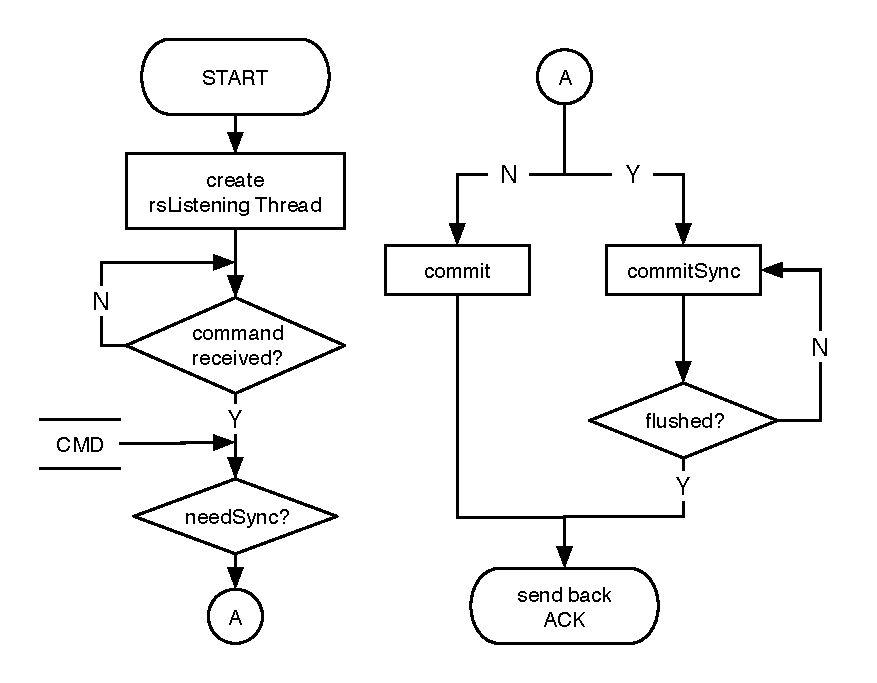
\includegraphics[scale=0.8]{fig/rsListeningThread_flowchart.eps}
	\caption{Flowchart of rsListening thread}
	\label{fig:rsListeningThread_flowchart}
\end{center-figure}

\section{Network Ready}
\label{s:NetworkReady}

Follow the thinking, we need a additional transport layers to make \RS{} network-ready, as we said in chapter \ref{c:intro}. To facilitate this, we add a thread in addtion to threads we mentions in section \ref{s:DesignChoices}. We name it \textit{RS Listening Thread}, it takes over received commands and commits them to the remote engine. We expose the implmentation details in section \ref{s:rsListeningThread}.

\section{Challenge}
\label{s:challenge}
With transport layer, we could send the command to another end. But the problem is, where is more appropriate to take send() action? A direct approach is putting send() right after commit(). We verify our idea by implementation, the idea is right in principle but there are some issues not considered.
\begin{enumerate}

\item Replicated Command
\item Command Synchronization 
\item Allocation of Command Queue
\item The Pointer in Arguments
\end{enumerate}

We describe our approach to solve these issues in the last four section of chapter \ref{c:implementation}.




